\section{Development of a Remote-APP}\label{sec:FrontendDev}
\textbf{AI Disclaimer}: AI was extensively used to generate  code for the App. The file structure, descriptions of main functions and architecture of the app as a whole were not designed by AI, because this information has laid down the groundwork for efficient use of AI to write this said code. Considering this, the chapter will not focus as much on code snippets with in-depth explanation of how the code functions, but rather on a structural overview and architecture of the project. File and app structure, most important functions and state selection will be covered here. The code provided by AI was reviewed and tested for its functionality, however it was not tested for the security (A common concern and weak spot of AI-Generated code), because of lack of such requirement and time constraints. Motivation and methodology for the use of AI will be discussed in the \hyperref[sec:discussion]{Results Analysis and Discussion} section.

Existence of a remote app is one of the main requirements and a hardest one. The problem here lies in the amount of choices one needs to do upfront, which also contributes to uncertainty about the extent of the project, which will be talked about in \hyperref[sec:discussion]{Results Section} in greater detail. For platform, Android was chosen. Alternatives were Web-based User Interface with Javascript+HTML or IOS. Android was chosen over WebUI or IOS solely from personal preference. A significant amount of time was also spent designing the structure of an app to make it ergonomic, to separate all the functions into different context windows.

The App is structurally subdivided into multiple parts: 
\begin{enumerate}
	\item \textbf{Bluetooth connection interface} (\texttt{\textbf{com.example.dispenser.ble}}) package Consists of 2 files: \textbf{BluetoothLeManager.kt} and \textbf{GattAttributes.kt}. 
	
	\textbf{BluetoothLeManager.kt} contains all the functions needed to establish bluetooth communication with the microcontroller using \ac{BLE} protocol, such as environment scan, dispenser identification, reading and writing data using \ac{BLE}.
	
	\textbf{GattAttributes.kt} contains all the \ac{UUID}s used by the microcontroller with names assigned to them, to avoid magic numbers in the code and replace them with named constants. This is a common practice everywhere, especially in microcontroller programming (where even a value of 0 is often rather depicted as LOW in the code, to avoid confusion)
	\item \textbf{User Interface} (\texttt{\textbf{com.example.dispenser.screens}}) package consists of 3 files that represent their assigned context windows:
	\begin{itemize}
		\item \textbf{DevConnScreen.kt} Contains the code for the UI of the "Device Connection" view. It contains the button to scan the environment for all the bluetooth devices, which are listed in the list under the \textbf{Found Devices}. At the very bottom there is also a connection status of the app to the device. When There is also a detection method (based on the device name) to detect the pill dispenser. The app will not attempt to connect to any other device.

		\item \textbf{DevConfScreen.kt} Contains the code for the UI of the "Device Configuration" view. It contains all the settings regarding the configuration of device, such as: Time of dispense, schedule template load/save, view current schedule, ability to edit or delete current schedule, as well as adding new schedule template and the schedule save/load indicator. It also contains the information about on-board clock and the ability to set or change it
		
		\item \textbf{DevMonitoringScreen.kt} Contains the code for the UI of the "Monitoring \& Status" view. It contains all the miscellaneous information about the device such as: Connection status, Last dispensed time, time until next dispense. The device logs are also available there. Logs contain information about bluetooth connection, information about past dispense events.
		
		\item \texttt{\textbf{com.example.dispenser.screens.devconnection}} package contains a class called \textbf{DevConnViewModel.kt} that contains functions related to updating the state of the connection view. It provides live update on information sent and received between the Device and the App, using \texttt{\textbf{\mbox{BluetoothLeManager}}}. 
		
		\item \texttt{\textbf{com.example.dispenser.ui.theme}} package defines the application style: colors, fonts, themes etc.
	\end{itemize}
	\item \texttt{\textbf{AndroidManifest.xml}} Declares information about the App: Permissions,  hardware requirements for the device, \textbf{MainActivity.kt} as an executive function (similar to main.c in C).
\end{enumerate}

The next section will cover in specific detail the initial requirements given to the AI to generate the code, as well as the results of the code review and how it actually functions.
\subsection{Bluetooth Connection Interface}\label{subsec:Bluetooth}
The requirements for bluetooth connection on the side of Android App are as follows:
\begin{enumerate}
	\item Scan for devices, identify the device that is a Pill Dispenser (using Name as an identificator)
	\item Connect to the device using \ac{BLE}
	\item Read Characteristics(\ac{GATT} Attributes): 
	\begin{itemize}
		\item \textbf{CHAR\_GET\_DEVICE\_TIME\_UUID} to get the current time set on the dispenser.
		\item \textbf{CHAR\_GET\_DISPENSE\_SCHEDULE\_UUID} to get the currently programmed dispense schedule from the dispenser.
		\item \textbf{CHAR\_GET\_LAST\_DISPENSE\_INFO\_UUID} to get information about the most recent dispense event
		\item \textbf{CHAR\_GET\_TIME\_UNTIL\_NEXT\_DISPENSE\_UUID} to get the remaining time until the next scheduled dispense.
		\item \textbf{CHAR\_GET\_DISPENSE\_LOG\_UUID} retrieve a log of past dispense events.
	\end{itemize}
	\item Write characteristics (Also \ac{GATT} Attributes):
	\begin{itemize}
		\item \textbf{CHAR\_SET\_DEVICE\_TIME\_UUID} to send the current time from the App to the dispenser.
		\item \textbf{CHAR\_SET\_DISPENSE\_SCHEDULE\_UUID} to send a new dispense schedule (time) to the dispenser.
		\item \textbf{CHAR\_TRIGGER\_MANUAL\_DISPENSE\_UUID} to send a command to make the dispenser dispense pills immediately.
	\end{itemize}
	\item Manually disconnect from device
\end{enumerate}
All these initial requirements were implemented in code. \ac{GATT} attributes form an interfacing protocol contract between the mobile application and the microcontroller. This shared definition ensures both systems can correctly interpret the \ac{BLE} services and characteristics. Consequently, these attributes are mirrored in the microcontroller's firmware, as detailed in Section  \hyperref[sec:Backenddev]{Microcontroller Programming}. As mentioned above, the Bluetooth connection interface consists of 2 files, \textbf{BluetoothLeManager.kt} and \textbf{GattAttributes.kt}. The first one contains all the functions and classes for the Backend-Frontend interface, while the second one contains \ac{GATT} attributes and their corresponding \ac{UUID}s. Code block \ref{lst:GATTs} is the full \textbf{GattAttributes.kt} file. This file contains all the Attributes that were present in the requirements, as well as some service attributes.
The standard way of defining it is \texttt{val NAME\_UUID: UUID = UUID.fromString("UUID")}, where \textbf{val} defines a read-only nature of the value (similar, but not quite the same as \texttt{const} keyword in C++), \textbf{UUID} = UUID... is the Java UUID class.



\begin{lstlisting}[style=kotlinstyle,caption={\ac{GATT} attributes defined in a separate file},label={lst:GATTs},float=htbp,language=Kotlin,numbers=left]
// GattAttributes.kt
package com.example.dispenser.ble

import java.util.UUID

object GattAttributes {
	// Service UUID
	val SERVICE_UUID: UUID = UUID.fromString("03339647-3f4e-43df-abff-fac54287cf1a")
	
	// Writable Characteristics
	val CHAR_SET_DEVICE_TIME_UUID: UUID = UUID.fromString("65232f1d-618a-4268-9050-0548142a4536")
	val CHAR_SET_DISPENSE_SCHEDULE_UUID: UUID = UUID.fromString("999c584e-06c0-49a1-995a-66b7c802ac1b")
	val CHAR_TRIGGER_MANUAL_DISPENSE_UUID: UUID = UUID.fromString("36bb95f2-e57e-4db9-b9aa-fb6541ee784e")
	
	// Readable Characteristics
	val CHAR_GET_DEVICE_TIME_UUID: UUID = UUID.fromString("272ee276-e37e-4d78-8c5e-bb7225d35074")
	val CHAR_GET_DISPENSE_SCHEDULE_UUID: UUID = UUID.fromString("b53c2ed4-ae26-476d-8414-011a025dddfc")
	val CHAR_GET_LAST_DISPENSE_INFO_UUID: UUID = UUID.fromString("40d3b5d8-5480-4b7b-a115-5fe86bf17d7d")
	val CHAR_GET_TIME_UNTIL_NEXT_DISPENSE_UUID: UUID = UUID.fromString("4b14acc4-768a-43e1-9d6c-0d97307e2666")
	val CHAR_GET_DISPENSE_LOG_UUID: UUID = UUID.fromString("6f182da7-c5a8-40ab-a637-f97ed6b5777b")
	
	// Descriptor for enabling notifications/indications
	val CLIENT_CHARACTERISTIC_CONFIG_UUID: UUID = UUID.fromString("00002902-0000-1000-8000-00805f9b34fb")
}
\end{lstlisting}
One interesting property of Kotlin as a programming language can be seen in this code. Line 4 contains an import of a Java library, this means that Kotlin is interoperable with Java and can use its libraries.

Moving forward, some properties of the Kotlin language need to be established:
\begin{enumerate}
	\item \textbf{Mutability}: References to immutable objects or variables cannot be changed once created. When modification appears to happen, a new object (with different reference) is created with the modification applied to new object only \cite{kotlin_variables} \cite{kotlin_collections}.
	\item \textbf{Null-safety}: default variable declaration forbids it to have a \texttt{null} value i.e. definition strictly follows declaration and memory gets immediately allocated to the variable. \textbf{Nullable} (i.e. those which are able to hold \texttt{null} value) can be created by appending a '?' symbol e.g.: \texttt{var b: String? = null}. It is  compile-time safety feature aimed at reduction of runtime Null-Pointer exceptions \cite{kotlin_null_safety}.
	\item \textbf{Coroutines and Flows} allow multithreading and simultaneous execution of multiple functions. Coroutines Provide means for writing asynchronous, non-blocking code in a sequential style \cite{kotlin_coroutines}. Flows are asynchronous data streams \cite{kotlin_flow}. 
	\item \textbf{StateFlow} is a special type of flow that is often used in the code below. It has 3 important Properties: State-Holder (always contains a value), Observable (all state collector functions receive information about state change of this object) and "Hot Flow" (A flow is hot because its active instance exists independently of the presence of collectors. This is opposed to a regular Flow, which is cold and is started separately for each collector)\cite{jetbrains_stateflow}.
	\item \textbf{Scope Functions (\texttt{let, run, with, apply, also})} allow execution of block of code within the context of a given object. Allow referring to an object in different ways and run operations with it as a reference \cite{kotlin_scope_functions}.
\end{enumerate}

\textbf{BluetoothLeManager.kt} Contains all the logic of the Android app related to interacting with the device. The code block \ref{lst:BLEman} is the top-level structure of the file. At the highest level there is package definition, library imports, service constant TAG used for logging and main. This file itself is too big (740 lines of code) to do an overview line-by-line and its exact functionality is not the scope of this thesis. In this case, a top level overview of the contents of the file will provide the context for understanding the project as a whole, without digging too deep in technical implementation, specifics of the language and the Platform and their interaction with \ac{BLE} protocol.

 \texttt{BluetoothLeManager} is a class that contains all functions and values for the interface. It relies heavily on built-in Android Package called \texttt{android.bluetooth} \cite{android_bluetooth}. 

The class takes 2 input parameters:
\begin{enumerate}
	\item \texttt{private val context: Context} to get the \texttt{BluetoothManager} (and subsequently the \texttt{BluetoothAdapter}) using \texttt{context.getSystemService(Context.BLUETOOTH\_SERVICE)} as an entry point to all Bluetooth operations. Consequently, also handles Permissions and \ac{GATT} connections.
	\item \texttt{private val coroutineScope: CoroutineScope} defines the lifecycle and context for any new coroutines launched within it. Since \ac{BLE} operations are asynchronous, this handles it by defining a coroutine on the Android side for each operation.
\end{enumerate} 
Next, within the class, objects meant for the correct function of \ac{BLE} are created:
\begin{itemize}
	\item \textbf{\_characteristicUpdate} is a private(visible only inside the class), mutable active flow. It's used internally by \texttt{BluetoothLeManager} to emit events when a characteristic's value is updated.
	\item \textbf{characteristicUpdate} is the public(visible outside the class), read-only version of \texttt{\_characteristicUpdate}. External classes can read flow information from this variable to be notified of characteristic value changes. \textbf{Note:} StateFlows are paired like that in the code, in the next instances where public and private instance of the same StateFlow are present, both of them will be described under the same bullet point
	\item \textbf{discoveredCharacteristics} is a private mutable map that stores the objects called \texttt{BluetoothGattCharacteristic} that are discovered on the connected peripheral. Values received from the Device are written within this variable.
	\item \textbf{bluetoothManager} is an instance of the Android Built-in \texttt{BluetoothManager} system service\cite{android_bluetooth}. This is the primary entry point for accessing Bluetooth functionality.
	\item \textbf{bluetoothAdapter} is the local device's Bluetooth adapter(hardware) object, also from built-in Android package \cite{android_bluetooth}. Nullable in case when a device with this App on it doesn't have Bluetooth. With this all standard Bluetooth operations, such as switching on, scanning and  connection can be made.
	\item \textbf{bleScanner} is an instance of BluetoothLeScanner(a method of built-in Android Bluetooth class) used specifically for scanning for \ac{BLE} devices. \texttt{by lazy} is a keyword indicating that this object(\texttt{blescanner}) will initialize only when its parent (\texttt{bluetoothAdapter?.bluetoothLeScanner})  is initialized.
	\item \textbf{scanJob} is a nullable(notice the '?' symbol) Coroutine Job used to manage the lifecycle of an ongoing BLE scan operation. Allows asynchronous scan operation to be started, monitored and cancelled.
	\item \textbf{connectJob} is a nullable Coroutine Job used to manage the lifecycle of an ongoing \ac{BLE} connection attempt. Allows asynchronous \ac{GATT} connection.
	\item \textbf{\_foundDevices} is private, mutable StateFlow that holds the current list of discovered \ac{BLE} devices. it gets internally updated by the \texttt{leScanCallback} as new devices are found during a scan. While the public version of it Exposes the list of discovered devices to the \texttt{DevConnViewModel}, which allows the UI to display found devices.
	\item \textbf{\_isScanning} is a private, mutable StateFlow indicating whether a scan is currently active. Used internally to track the scanning state and prevent multiple concurrent scans. Public version of it allows the UI to observe the current scanning status.
	\item \textbf{\_connectionStatus} is a private, mutable StateFlow which holds the current connection status (e.g., Disconnected, Connecting, Connected, Error). Used internally to reflect the real-time state of the \ac{BLE} link. Public version of it allows UI to display the current connection status and to make decisions based on this state (e.g., enabling/disabling certain actions).
	\item \textbf{\_connectedDevice} A private, mutable StateFlow, it holds information not only about whether a device is connected, but also about the currently connected device. Public version of it Allows the UI to know which device is currently connected.
	\item \textbf{currentGatt} is a nullable instance of built-in android BluetoothGatt class from the android.bluetooth package\cite{android_bluetooth} that provides \ac{GATT} client functionality. When a device is not connected, this class can be \texttt{null}. It is a main object of all interactions with connected device.
\end{itemize}
The next 3 functions are made for permission checks:
\begin{itemize}
	\item \textbf{hasPermission} is an utility function to check if a specific permission (passed as a String) has been granted to the application.
	\item \textbf{hasRequiredScanPermissions} Checks if all necessary permissions for \ac{BLE} scanning are granted. It also contains security features that prevent the App from asking for permissions that might not exist on the device (e.g. when Android version is too old).
	\item \textbf{hasRequiredConnectPermissions} Serves the same purpose as function above, but this time for connection permissions.
\end{itemize}
The following two functions and one object handle the scanning function of the App:
\begin{itemize}
	\item \textbf{startScan} is a function that initiates a scan to discover all advertising devices in the reach. It performs permission checks,  Checks if Bluetooth is enabled, Sets \texttt{\_isScanning} to true and clears \texttt{\_foundDevices}, Starts the scan, Launches a \texttt{scanJob} to manage the scan, including a timeout (30 seconds) after which the scan is automatically stopped and finally, Updates \texttt{\_connectionStatus} with an error if prerequisites are not met.
	\item \textbf{stopScan} is a function that Stops an ongoing BLE scan. It Checks if a scan is actually in progress, Calls \texttt{bleScanner?.stopScan} using the \texttt{leScanCallback}, Sets \texttt{\_isScanning} to \textbf{FALSE}, Cancels the \texttt{scanJob} and finally, if there is an error during the stopping process, Handles potential Exceptions during the stop operation. 
	\item \textbf{leScanCallback} is an instance of \texttt{ScanCallback} class provided by the bluetooth.le package (it is different package that is made specifically for \ac{BLE} connection) \cite{android_bluetooth_le}. Its methods are invoked by the system when scan events occur. Using this class, device filtering is handled. If scan detects a device called "PillDispenserESP32" it will be marked with the \texttt{isPillDispenser} flag, outlining it and putting it at the top of the list of scanned devices.
\end{itemize}
The next functions handle the connection logic:
\begin{itemize}
	\item \textbf{connectToDevice} is a function that Initiates a \ac{GATT} connection to a \ac{BLE} peripheral specified by its \ac{MAC} address. First, it performs permission and bluetooth availability checks, then retrieves the \texttt{BluetoothDevice} object using the provided address, then launches a \texttt{connectJob} to handle the asynchronous connection process and finally, calls \texttt{deviceToConnect.connectGatt()} with the \texttt{gattCallback} to establish the connection.
	\item \textbf{disconnect} is a function that disconnects from the currently connected \ac{BLE} peripheral and closes the \ac{GATT} client. First, it checks if \texttt{currentGatt} is not null i.e. it is connected, then it performs permission checks, afterwards it calls the command \texttt{currentGatt?.disconnect()}, however the actual disconnection and resource cleanup (closing \ac{GATT}) are typically handled in the \texttt{onConnectionStateChange} callback and finally it  Cancels the \texttt{connectJob} if it was related to an ongoing connection attempt.
	\item \textbf{writeCharacteristic} function is used to write into the writable characteristics on the device. First, it checks for connect permissions and if \texttt{currentGatt} is valid. Then, retrieves the \texttt{BluetoothGattCharacteristic} from \texttt{discoveredCharacteristics}, so that it will know what writable characteristics are on the device. Then, it verifies that the characteristic supports the specified writeType (verifies that it is writable), calls \texttt{currentGatt?.writeCharacteristic()} and finally, if the write operation has successfully been initiated, it returns \textbf{TRUE}.
	\item \textbf{readCharacteristic} is in nature very similar to \texttt{writeCharacteristic}, but for read-only characteristics on the device. First, it checks for connect permissions and retrieves \texttt{BluetoothGattCharacteristic} (same as previous function), then verifies the read-only property of the characteristic,  Calls \texttt{currentGatt?.readCharacteristic()} and finally, returns \textbf{TRUE} if read operation was initiated successfully.
	\item \textbf{setCharacteristicNotificationEnabled} is a function that enables or disables notifications (or indications) for a given characteristic. Currently implemented, but not used, might be used for debugging and fine-tuning notifications.
	\item \textbf{enableNotificationsFor} is a private helper function specifically called during the \texttt{onServicesDiscovered} phase. This is a function that is more simple and robust than the one above. It centralizes the logic for enabling notifications for all relevant "GET\_..." characteristics as soon as they are discovered, simplifying the connection setup process
\end{itemize}
The next object is a key component for the functionality of the whole \ac{BLE} communication logic. 

\textbf{gattCallback} is an instance of built-in Android class called \texttt{BluetoothGattCallback}\cite{android_bluetooth} provided to the \texttt{connectGatt} method. This is the heart of managing an active \ac{BLE} connection and its asynchronous events. To accomplish this task, the class has methods built in it:
\begin{itemize}
	\item \textbf{onConnectionStateChange} is called when the connection state changes. If connected successfully, it triggers service discovery(\texttt{gatt?.discoverServices()}), on disconnection, it closes the \ac{GATT} client.
	\item \textbf{onServicesDiscovered} is called after \texttt{discoverServices()} completes. If successful, it iterates through the services and characteristics of the connected device. It populates the \texttt{discoveredCharacteristics} list with relevant characteristics defined in \texttt{GattAttributes} (SET/GET/TRIGGER UUIDs). It also calls \texttt{enableNotificationsFor()} function for readable characteristics to automatically subscribe to updates. If the required service or critical characteristics are not found, it updates \texttt{\_connectionStatus} to an error and disconnects.
	\item \textbf{onCharacteristicRead} is called when a characteristic read operation completes. 
	\item \textbf{handleCharacteristicRead} If the read was successful (GATT\_SUCCESS), it emits the characteristic's \ac{UUID} and value to the \texttt{\_characteristicUpdate} flow.
	\item \textbf{onCharacteristicWrite} Called after a characteristic write operation completes. Logs the success or failure. If failed, updates \texttt{\_connectionStatus} with an error.
	\item \textbf{onCharacteristicChanged} is called when the peripheral sends a notification or indication for a characteristic to which the client has subscribed. 
	\item \textbf{handleCharacteristicChanged} is a method that emits the characteristic's \ac{UUID} and updated value to the \texttt{\_characteristicUpdate} flow.
	\item \textbf{onDescriptorWrite} is called after a descriptor write operation completes (e.g. to enable/disable notifications). It logs the outcome.
\end{itemize}
The final function of the class is \textbf{cleanup} function. It releases all resources used by the \texttt{BluetoothLeManager}. this function is called when the model is no longer needed. it resets all states related to Bluetooth to their default state (disconnected, not scanning).
\begin{lstlisting}[
	style=kotlinstyle,
	caption={Top level structure of the BluetoothLeManager.kt file},
	label={lst:BLEman},
	language=Kotlin,
	numbers=left
	]
	package com.example.dispenser.ble
	import . . .
	private const val TAG = "BluetoothLeManager"
	
	class BluetoothLeManager(private val context: Context, private val coroutineScope: CoroutineScope)
	{
		private val _characteristicUpdate = MutableSharedFlow<Pair<UUID, ByteArray>>()
		val characteristicUpdate: SharedFlow<Pair<UUID, ByteArray>> = _characteristicUpdate.asSharedFlow()
		
		private val discoveredCharacteristics = mutableMapOf<UUID, BluetoothGattCharacteristic>()
		
		private val bluetoothManager = context.getSystemService(Context.BLUETOOTH_SERVICE) as BluetoothManager
		private val bluetoothAdapter: BluetoothAdapter? = bluetoothManager.adapter
		private val bleScanner by lazy { bluetoothAdapter?.bluetoothLeScanner }
		
		private var scanJob: Job? = null
		private var connectJob: Job? = null
		
		private val _foundDevices = MutableStateFlow<List<UiBluetoothDevice>>(emptyList())
		val foundDevices: StateFlow<List<UiBluetoothDevice>> = _foundDevices.asStateFlow()
		
		private val _isScanning = MutableStateFlow(false)
		val isScanning: StateFlow<Boolean> = _isScanning.asStateFlow()
		
		private val _connectionStatus = MutableStateFlow<ConnectionStatus>(ConnectionStatus.Disconnected)
		val connectionStatus: StateFlow<ConnectionStatus> = _connectionStatus.asStateFlow()
		
		private val _connectedDevice = MutableStateFlow<UiBluetoothDevice?>(null)
		val connectedDevice: StateFlow<UiBluetoothDevice?> = _connectedDevice.asStateFlow()
		
		private var currentGatt: BluetoothGatt? = null
		
		// Helper functions for permission checking
		private fun hasPermission(permission: String): Boolean
		private fun hasRequiredScanPermissions(): Boolean
		private fun hasRequiredConnectPermissions(): Boolean
		
		// Scan logic
		fun startScan()
		fun stopScan()
		private val leScanCallback = object : ScanCallback { ... }
		
		// Connection logic
		fun connectToDevice(deviceAddress: String)
		fun disconnect()
		
		// Characteristic operations
		fun writeCharacteristic(characteristicUUID: UUID, value: ByteArray, writeType: Int = ...): Boolean
		fun readCharacteristic(characteristicUUID: UUID): Boolean
		fun setCharacteristicNotificationEnabled(characteristicUUID: UUID, enable: Boolean): Boolean
		
		// Notification helper
		private fun enableNotificationsFor(characteristic: BluetoothGattCharacteristic)
		
		// GATT callback
		private val gattCallback = object : BluetoothGattCallback { ... }
		
		// Cleanup
		fun cleanup()
		
	}
\end{lstlisting}
\newpage
\subsection{User Interface}
Having finished with describing how the App handles interface between microcontroller using \ac{BLE}, the \ac{GUI} of the app will be covered next. It consists of 3 main views (called \textbf{Device Connection, Device Configuration and Monitoring \&  Status}), each of them contains different information and functions. Switching between views is done via a drawer panel on the left-hand side of the app, which slides open when the button at the top left is pressed.

Once again, before moving forward, there is a certain terminology that needs to be covered. This thesis uses terminology used by official design guide\cite{android_ui_layer} from \textbf{Android Developers} team, which is an industry standard.
\begin{itemize}
	\item \textbf{Jetpack Compose} while not a technical term as the others are on the list, Jetpack Compose is the modern toolkit for building native Android \ac{UI}. It defines the paradigm under which all the other terms operate.
	\item \textbf{ViewModel} class is a business logic or screen level state holder. Its principal advantage is that it caches state and persists it through configuration changes. The alternative to a ViewModel is a plain class that holds the data displayed in the \ac{UI}. This can become a problem when navigating between activities or Navigation destinations. Doing so destroys that data if it isn't stored using the saving instance state mechanism. 
	\item \textbf{ViewModelFactory} is a class responsible for creating instances of ViewModels. It's needed because ViewModels often have dependencies that need to be provided to them when they are created.
	\item \textbf{UI State} represents what to show on the screen. For the Device Connection screen, this includes whether the app is currently scanning, the list of found Bluetooth devices, the current connection status (e.g., "Disconnected", "Connecting", "Connected"), and any error messages. This state typically lives in or is managed by the ViewModel.
	\item \textbf{Composable Function (or "Composable")} This is the fundamental building block of \ac{UI} in Jetpack Compose. Instead of traditional XML layouts, \ac{UI} is defined by writing functions annotated with @Composable. These functions describe what the \ac{UI} should look like for a given state, not how to construct it step-by-step.
	\item \textbf{Recomposition} is the process of Jetpack Compose re-running Composable functions when their input \textbf{State} changes. If the \texttt{scanStatus} (part of the \ac{UI} State) changes from "Disconnected" to "Scanning", Compose will re-run (recompose) only the parts of \ac{UI} that depend on \texttt{scanStatus}, updating them automatically. \ac{UI} elements don't need to be manually updated.
	\item \textbf{Layout Composables (Column, Row, Box)} are special Composables used to arrange other Composables on the screen. Column arranges its children vertically, Row horizontally, and Box allows stacking elements or positioning them relative to its edges.
	\item \textbf{Event Handling (Callbacks/Lambdas)} is based on user interaction with \ac{UI}. Composables can trigger actions. This is usually done by passing lambda functions (callbacks) as parameters to the Composables.
	\item \textbf{StateFlow} has already been defined in the \hyperref[subsec:Bluetooth]{Bluetooth Connection} Section. It is a state-holder observable "hot" flow that always has a value and emits updates to its collectors. This term is even more important here, as it creates a bridge for understanding how User Interface interacts with data. In context of User Interface, it is is a primary mechanism for the \textbf{ViewModel} to expose \ac{UI} \textbf{State} to the Composable. Composable functions can observe (or "collect") these StateFlows, When the StateFlow emits a new value, collectAsState() receives this update and signals to the Compose runtime that the state read by a Composable has changed.
\end{itemize}
The Main entry file to the whole app is called \textbf{MainActivity.kt}. The fundamental part of the \ac{UI} is connected through this file. It is worth reviewing it here before delving deeper into the each view. The top level structure of the code can be seen in code block here \ref{lst:MainActivity}.

Main application structure is defined in the \textbf{AppScaffoldWithDrawer} composable function. It contains top app bar, a navigation drawer, and the main content area where different views are displayed. This function is called within the \texttt{MainActivity} class's \texttt{onCreate} method to set up the UI.
\texttt{AppScaffoldWithDrawer} has numerous tasks:
\begin{enumerate}
	\item \textbf{Navigation:} Manages the ModalNavigationDrawer to allows switching between different sections of the app ("Device Connection", "Device Configuration", "Monitoring \& Status").
	\item \textbf{Screen Switching:} Uses a \texttt{when} (similar to \texttt{case} and \texttt{switch} commands in C/C++) statement to display the appropriate screen in the Scaffold's content area.
	\item \textbf{ViewModel Access:} It receives the \texttt{devConnViewModelFactory} and uses it to obtain an instance of \texttt{DevConnViewModel}. This \texttt{ViewModel} is then passed down to the relevant screens.
	\item \textbf{Conditional UI:} It conditionally renders content within the "Device Connection" screen path(e.g. Popups that prompt granting permissions and enabling Bluetooth).
	\item \textbf{Callbacks:} Passes down callbacks to \texttt{MissingPermissionsScreen} and \\ \texttt{BluetoothDisabledScreen}.
\end{enumerate}
Besides \texttt{AppScaffoldWithDrawer} function, there are also various supplementary functions:
\begin{itemize}
	\item \textbf{MissingPermissionsScreen} is a simple UI screen displayed when the necessary Bluetooth permissions have not been granted by the user.It provides a "Grant Permissions" button that triggers the \texttt{onRequestPermissions} callback (which is implemented in \texttt{MainActivity}) to launch the permission request.
	\item \textbf{BluetoothDisabledScreen} is similar to \texttt{MissingPermissionsScreen}, but for when Bluetooth is disabled. Also provides an "Enable Bluetooth" button to switch it on.
	\item \textbf{DeviceConfigurationScreen} This is a legacy device configuration view, left from older iterations of the code. Currently not used, still left because it might be used for debugging. Device configuration view is currently handled in a separate file \texttt{DevConfScreen.kt}
	\item \textbf{MonitoringStatusScreen} Same as above, legacy view for Device Monitoring \& Status screen, currently not used. This View is currently handled by \texttt{DevMonitroingScreen.kt} file.
	\item \textbf{AppScaffoldWithDrawerPreview} is an assistance function for Prototyping. Android Studio has built-in app preview functionality, this helper function allows seeing how \texttt{AppScaffoldWithDrawer} looks without running the entire app on an emulator or device.
\end{itemize}
Next, \texttt{MainActivity} class ought to be reviewed next. It is a primary \texttt{Activity} of the application, handles lifecycle, Compose \ac{UI} and manages permissions and Bluetooth initialization.
It has 3 parameters:
\begin{itemize}
	\item \textbf{private val applicationScope} is a \texttt{CoroutineScope} that lives as long as \texttt{MainActivity} is explicitly active. It consists of 2 components: \texttt{SupervisorJob} ensures that if one child coroutine fails, others are not cancelled. \texttt{Dispatchers.Default} is used for CPU-intensive work off the main thread.
	\item \textbf{private lateinit var bluetoothLeManager} holds the instance of \texttt{BluetoothLeManager}, the class that was extensively covered in the \hyperref[subsec:Bluetooth]{Bluetooth Connection} Section.
	\item \textbf{private val blePermissions} is used to define an array of Bluetooth-related permissions required by the app, adapting to different Android versions (API 31/Android S and above have different permission requirements). Necessary for compatibility with older devices that have a different set of permissions.
\end{itemize}
Then, it has 4 different methods, each serving different purpose:
\begin{itemize}
	\item \textbf{onCreate} is a Lifecycle method, which is called when activity is starting. It fulfills many important tasks: Initializes the \texttt{BluetoothLeManager}. Using \texttt{setContent \{ ... \}} it creates entry point for Jetpack Compose, which defines the UI content. Besides that, it also sets the stage for the function of the app as a whole: it establishes \textbf{Permission Handling, Bluetooth Enabled Checking, Initial Permission/Bluetooth Requests, ViewModel Factory Creation} and finally \textbf{Main UI Setup}. 
	\item \textbf{checkAllPermissionsGranted} is a private helper method  that serves as a checklist to go through and check if all permissions (defined in \texttt{blePermissions}) have been granted. It initializes \texttt{hasPermissions} on creation from method above and can be called again to re-check permissions.
	\item \textbf{isBluetoothAdapterEnabled} is a private helper method that checks if Bluetooth adapter is currently enabled. It initializes \texttt{isBluetoothEnabled} in \texttt{OnCreate} and by \texttt{enableBluetoothLauncher} to check if Bluetooth is enabled.
	\item \textbf{onDestroy} is a lifecycle method for termination of the task that is used to release resources. It works together with the \texttt{bluetoothLeManager.cleanup()} method from the BluetoothLeManager class to clean up  the resources.
\end{itemize}
\begin{lstlisting}[
	style=kotlinstyle,
	caption={Top-level structure of the \texttt{MainActivity.kt} file},
	label={lst:MainActivity},
	language=Kotlin,
	numbers=left
	]
	package com.example.dispenser
	import . . .
	
	class MainActivity : ComponentActivity() {
		
		private val applicationScope = CoroutineScope(/* SupervisorJob() + Dispatchers.Default */)
		private lateinit var bluetoothLeManager: BluetoothLeManager   // Instantiate early
		
		// List of permissions
		private val blePermissions =
		if (Build.VERSION.SDK_INT >= Build.VERSION_CODES.S) { ... } else {
			arrayOf(
			Manifest.permission.BLUETOOTH,
			Manifest.permission.BLUETOOTH_ADMIN,
			Manifest.permission.ACCESS_FINE_LOCATION   // or coarse
			)
		}
		
		// Lifecycle
		override fun onCreate(savedInstanceState: Bundle?) { ... }
		private fun checkAllPermissionsGranted(): Boolean
		private fun isBluetoothAdapterEnabled(): Boolean
		override fun onDestroy() { ... }
	}
	
	/* ---------- Composables ---------- */
	
	@OptIn(ExperimentalMaterial3Api::class)
	@Composable
	fun AppScaffoldWithDrawer(
	modifier: Modifier = Modifier,
	permissionsGranted: Boolean,
	isBluetoothEnabled: Boolean,
	onRequestPermissions: () -> Unit,
	onRequestEnableBluetooth: () -> Unit,
	devConnViewModelFactory: DevConnViewModelFactory
	) { ... }
	
	@Composable
	fun MissingPermissionsScreen(onRequestPermissions: () -> Unit) { ... }
	
	@Composable
	fun BluetoothDisabledScreen(onRequestEnableBluetooth: () -> Unit) { ... }
	
	// Place-holder composables for future screens
	@Composable
	fun DeviceConfigurationScreen() { ... }
	
	@Composable
	fun MonitoringStatusScreen() { ... }
	
	/* ---------- Preview ---------- */
	@Preview(showBackground = true)
	@Composable
	fun AppScaffoldWithDrawerPreview() { ... }
\end{lstlisting}

\subsubsection{Device Connection}
\begin{figure}[h!]
	\centering
	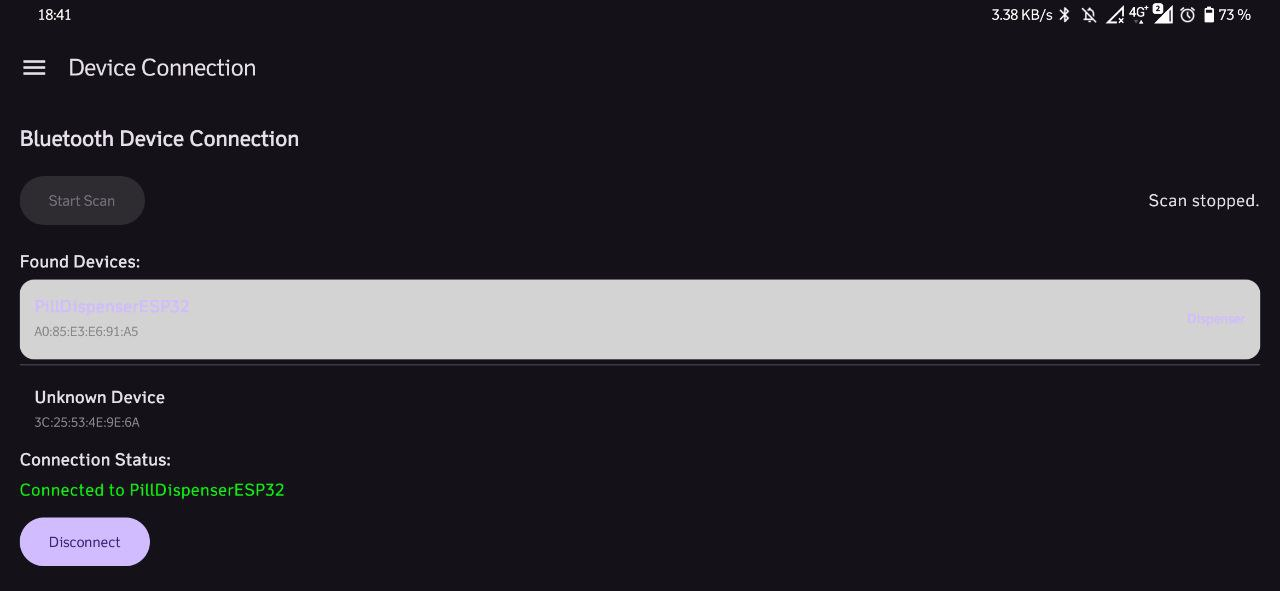
\includegraphics[width=0.8\linewidth]{Figures/devConnView}
	\caption[Device connection view.]{Device connection view.}
	\label{fig:devconnview}
\end{figure}
The structure behind \textbf{Device Connection} view consist of multiple files that contribute to this view:
\begin{enumerate}
	\item \textbf{DevConnScreen.kt} file contains the Composable function \texttt{DevConnScreen}, which defines the visual layout and user interface elements for the device connection screen.
	\item \textbf{DevConnViewModel.kt} file contains State management logic. It acts as a bridge between the UI (\texttt{DevConnScreen}) and the data layer (\texttt{BluetoothLeManager}). It holds the state displayed by the UI and processes user actions.
	\item \textbf{BluetoothLeManager.kt} Covered in previous section, is a class responsible for handling \ac{BLE} interactions between Device, Android Bluetooth \ac{API} and \ac{GUI}.
	\item \textbf{MainActivity.kt} is the main entry point of this app. It sets up the overall UI structure, including the navigation drawer and the content area where all the screens are displayed.
	\item \textbf{DevConnViewModelFactory.kt} is a standard ViewModel factory responsible for creating instances of \texttt{DevConnViewModel}
	\item \textbf{GattAttributes.kt} Defines the unique UUIDs for \ac{BLE} service and characteristics on the ESP32. Already covered in the \hyperref[subsec:Bluetooth]{Bluetooth Connection} Section.
\end{enumerate}
Many of these files (\textbf{BluetoothLeManager.kt}, \textbf{MainActivity.kt} and \textbf{GattAttributes.kt}) have already been previously covered and 3 files that we will cover next, to understand how the view is created.
\newpage
\textbf{DevConnScreen.kt} file is responsible for layout and \ac{UI} elements. Its top level structure can be seen in code block \ref{lst:DevConnVM} It contains:
\begin{itemize}
	\item \textbf{UiBluetoothDevice} data class serves as a simplified representation of a Bluetooth device, made to be displayed in the \ac{UI}. It's more convenient to use this in Composable functions than the raw Android \texttt{BluetoothDevice} object directly. Instances of this class are used to populate the list of found devices displayed on the screen(\ac{MAC} address, Device name and whether it is a Pill Dispenser).
	\item \textbf{ConnectionStatus} class defines a set of distinct states representing the current status of the Bluetooth scanning and connection process. It is a \textbf{sealed} class, which means that all direct subclasses of a sealed class must be declared in the same file as the sealed class itself. Here it is used for a state-switch (using an already known command \texttt{when}). It has 4 state objects: \texttt{Disconnected, Scanning, Connecting, Connected}, each representing current relationship of an App to the device.
	\item \textbf{DevConnScreen} is a primary composable function that defines the entire layout and behavior of the \textbf{Device Connection} screen. It is quite vast function in a sense that through it the whole view is displayed, therefore it is worth documenting it deeper. \texttt{DevConnScreen} takes many input parameters:
	\begin{itemize}
		\item \textbf{scanStatus} is the current status of the scanning process
		\item \textbf{foundDevices} is list of discovered Bluetooth devices.
		\item \textbf{connectionStatus} is current status of the device connection.
		\item \textbf{connectingDevice} is the device that is currently being connected to, or is already connected.
		\item \textbf{lastError} general error message that might not be part of either  \texttt{scanStatus} or \texttt{connectionStatus}
		\item \textbf{onStartScanClick} is a callback function invoked when the "Start Scan" button is clicked.
		\item \textbf{onStopScanClick} is a callback function invoked when the "Stop Scan" button is clicked.
		\item \textbf{onDeviceClick} is a callback function invoked when a device in the list is clicked.
		\item \textbf{onDisconnectClick}is a callback function invoked when the "Disconnect" button is clicked.
	\end{itemize}
	In essence, this function is responsible for every element of the \ac{UI} seen within the "Device Connection Screen" window.
	\item \textbf{DeviceListItem} is a helper Composable function responsible for rendering a single item in the list of found Bluetooth devices. In essence, this function is responsible for the contents of a single card from the list of scanned devices. It is called each time a new device is found to draw a card with information about this device within it.
	\item \textbf{DevConnScreenPreview\_*} are multiple functions with similar names and purpose. Each of them serves the debugging previewing, allowing checking different states of this window within Android Studio without having to compile and emulate the whole app.
\end{itemize}

\textbf{DevConnViewModel.kt} is responsible for State management. It contains:
\begin{itemize}
	\item \textbf{DevConnViewModel} class is a ViewModel designed to manage the UI-related data for the device connection screen. It is also worth noting that this ViewModel is used by other views that interact with the connected \ac{BLE} device. It inherits from Android built-in \texttt{AndroidViewModel}, which provides it with an Application context, useful for system services or application-wide resources.
	\item \textbf{scanStatus} is a StateFlow exposes the current status of the BLE scanning process to the UI.
	\item \textbf{foundDevices} is a StateFlow that exposes the current status of the connection to a BLE device. 
	\item \textbf{connectingDevice} is a Stateflow that covers the specific device that is currently in the process of connecting or is already connected. It is nullable, therefore it can also be \texttt{null} if no device is connected.
	\item \textbf{\_lastError} is a private, mutable state holder for any general error messages that the ViewModel itself might generate. Nullable, and is \texttt{null} when initialized.
	\item  \textbf{displayError} is a StateFlow that Provides a single, consolidated error message for the UI. 
	\item \textbf{startScan(), stopScan(), connectToDevice(device: UiBluetoothDevice) and disconnect()} are functions managing interaction with the deivce. They use corresponding methods from the \texttt{BluetoothLeManager} class.
	\item \textbf{setGeneralError} is a helper function to allow setting a custom error message to \textbf{\_lastError}
\end{itemize}
The next StateFlows within the \texttt{DevConnViewModel} class are related to interaction with Timer/Counter of the device, which plays a pivotal role in its configuration and interaction in general
\begin{itemize}
	\item \textbf{\_deviceTime} is a StateFlow that holds the current time of the connected device, as a string. \textbf{deviceTime} is a similar non-mutable StateFlow to display the time in \ac{UI}.
	\item \textbf{\_dispenseSchedule} is a StateFlow that contains the current dispense schedule of the connected dispenser device, as a string. \textbf{dispenseSchedule} is an immutable variant of this.
	\item \textbf{\_lastDispenseInfo} Holds information about the last dispense event from the dispenser. \textbf{lastDispenseInfo} is an immutable variant.
	\item \textbf{\_timeUntilNextDispense} Holds the calculated or received time until the next scheduled dispense. \textbf{timeUntilNextDispense} is an immutable variant.
	\item \textbf{\_dispenseLog} Holds a log of dispense events from the dispenser. \textbf{dispenseLog} is an immutable variant.
\end{itemize}

The next code block \textbf{init \{. . .\}} is executed when an instance of \texttt{DevConnViewModel} is created. It is used to set up long-lived operations or observers. It launches a coroutine in \texttt{viewModelScope} to collect connection data from \texttt{bluetoothLeManager.connectionStatus}. If the status is not Connected, it resets all the device-specific data (\texttt{\_deviceTime, \_dispenseSchedule,} etc.) to their "N/A (Disconnected)" states.

After this block, functions related to sending data from the App to the device are defined:
\begin{itemize}
	\item \textbf{triggerManualDispense} sends a command to the connected BLE device to perform a manual dispense.
	\item \textbf{setDeviceTime} sends a command to the connected BLE device to set its internal time.
	\item \textbf{setDispenseSchedule} sends a command to the connected BLE device to set its dispense schedule.
	\item \textbf{requestDeviceTime} sends a request to the connected BLE device to read its current time characteristic.
	\item \textbf{requestDispenseSchedule} sends a request to read the dispense schedule characteristic.
	\item \textbf{requestLastDispenseInfo} sends a request to read the last dispense info characteristic.
	\item \textbf{onCleared} This method is called when the ViewModel is no longer used and is about to be destroyed. It's the place to clean up any resources tied to the ViewModel's lifecycle.
\end{itemize}

\begin{lstlisting}[
	style=kotlinstyle,
	caption={Top-level structure of the \texttt{DevConnViewModel.kt} file},
	label={lst:DevConnVM},
	language=Kotlin,
	numbers=left
	]
	package com.example.dispenser.screens.devconnection
	
	import ...
	
	class DevConnViewModel(
	application: Application,
	private val bluetoothLeManager: BluetoothLeManager
	) : AndroidViewModel(application) {
		
		// State for scan status (now reflects manager's scanning state)
		val scanStatus: StateFlow<ConnectionStatus> = bluetoothLeManager.isScanning
		.map { isScanning ->
			if (isScanning) ConnectionStatus.Scanning else ConnectionStatus.Disconnected
		}
		.stateIn(viewModelScope, SharingStarted.Lazily, ConnectionStatus.Disconnected)
		
		// State for found devices (directly from manager)
		val foundDevices: StateFlow<List<UiBluetoothDevice>> = bluetoothLeManager.foundDevices
		
		// State for device connection status (directly from manager)
		val connectionStatus: StateFlow<ConnectionStatus> = bluetoothLeManager.connectionStatus
		
		// State for the device currently being connected to/connected (directly from manager)
		val connectingDevice: StateFlow<UiBluetoothDevice?> = bluetoothLeManager.connectedDevice
		
		// State for any last error message (can be a combination or specific errors)
		// For now, let's use the connectionStatus error or a general one.
		private val _lastError = MutableStateFlow<String?>(null) // For other types of errors if needed
		val lastError: StateFlow<String?> = _lastError.asStateFlow()
		
		// Combine scan errors and connection errors into a displayable error
		val displayError: StateFlow<String?> = combine(
		bluetoothLeManager.connectionStatus, // For connection/scan errors from manager
		_lastError // For other general errors set by ViewModel
		) { connStatus, generalError ->
			if (connStatus is ConnectionStatus.Error) {
				connStatus.message
			} else {
				generalError
			}
		}.stateIn(viewModelScope, SharingStarted.Eagerly, null)
		
		fun startScan() { ... }
		fun stopScan() { ... }
		fun connectToDevice(device: UiBluetoothDevice) { ... }
		fun disconnect() { ... }
		fun setGeneralError(message: String?) { ... }
		
		private val _deviceTime = MutableStateFlow<String?>("N/A")
		val deviceTime: StateFlow<String?> = _deviceTime.asStateFlow()
		
		private val _dispenseSchedule = MutableStateFlow<String?>("N/A")
		val dispenseSchedule: StateFlow<String?> = _dispenseSchedule.asStateFlow()
		
		private val _lastDispenseInfo = MutableStateFlow<String?>("N/A")
		val lastDispenseInfo: StateFlow<String?> = _lastDispenseInfo.asStateFlow()
		
		private val _timeUntilNextDispense = MutableStateFlow<String?>("N/A")
		val timeUntilNextDispense: StateFlow<String?> = _timeUntilNextDispense.asStateFlow()
		
		private val _dispenseLog = MutableStateFlow<String?>("N/A")
		val dispenseLog: StateFlow<String?> = _dispenseLog.asStateFlow()
		init { ... }
		fun triggerManualDispense() { ... }
		fun setDeviceTime(timeString: String) { ... }
		fun setDispenseSchedule(scheduleString: String) { ... }
		fun requestDeviceTime() { ... }
		fun requestDispenseSchedule() { ... }
		fun requestLastDispenseInfo() { ... }
		override fun onCleared() { ... }
	}
\end{lstlisting}
And Finally, \textbf{DevConnViewModelFactory.kt} file contains contains a single \textit{DevConnViewModelFactory} class. It is a custom factory responsible for creating instances of \texttt{DevConnViewModel} This is necessary because \texttt{DevConnViewModel} requires arguments in its constructor (\texttt{application} and \texttt{bluetoothLeManager}), which the default ViewModel provider mechanism cannot supply.
\subsubsection{Device Configuration}
  a. Add/Configure Dispense Schedule:
  i. Time of dispense (up to 3 a day). Get current timer/Clock
  ii. Save/Load Schedule. Stored in android app
  
  b. View Current Schedule:
  i. Display a clear list of all programmed dispense times and associated details. (Parse T/C info into Calendar info)
  
  c. Edit/Delete Schedule:
  i. Allow modification of existing schedules (time, days, name).
  ii. Allow removal of unneeded schedules.
  iii. (Important) Ensure changes are reliably sent and confirmed by the dispenser hardware. (ESP32/App T/C Matching)
  
  d. Configure Device Time Get current Clock/Set Current Clock
  
\subsubsection{Monitoring \&  Status}

a. Device Status Display:
i. Show basic status received from the dispenser:
1. Connected/Disconnected
2. Battery Level (ESP32 Function)
3. Last dispensed time/status (Success/Failure) (Requires Sensor) (Sensor+T/C info)
4. Current time on the dispenser (to check sync) T/C Info
5. Time until next dispense T/C Info

b. Dispense History/Log:
i. Display a log of past dispense events. (Need to configure Logging storage on ESP32, last 30 due to small memory size)
ii. Information per entry: Timestamp, Scheduled Time, Medication Name (if set), Status (e.g., Dispensed Successfully, Failed, Skipped). This is crucial for tracking adherence.
